\documentclass[12pt, twoside]{article}
\usepackage[letterpaper, margin=1in, headsep=0.5in]{geometry}
\usepackage[english]{babel}
\usepackage[utf8]{inputenc}
\usepackage{amsmath}
\usepackage{amsfonts}
\usepackage{amssymb}
\usepackage{tikz}
\usetikzlibrary{quotes, angles}
\usepackage{graphicx}
\usepackage{enumitem}
\usepackage{multicol}

\newif\ifmeta
\metatrue %print standards and topics tags

\title{Regents Geometry}
\author{Chris Huson}
\date{October 2021}

\usepackage{fancyhdr}
\pagestyle{fancy}
\fancyhf{}
\renewcommand{\headrulewidth}{0pt} % disable the underline of the header
\raggedbottom


\fancyhead[LE]{\thepage}
\fancyhead[RO]{\thepage \\ Name: \hspace{4cm} \,\\}
\fancyhead[LO]{BECA / Dr. Huson / Geometry 03 Parallels and transversals}

\begin{document}

\subsubsection*{3.5 Exit Note: Fractions and notation}
\begin{enumerate}
\item Given $\overline{DEFG}$, $DE=3 \frac{1}{2}$, $EF=7 \frac{1}{2}$, and $FG= 2 \frac{1}{2}$. (diagram not to scale)\\ [0.25cm]
  Find ${DG}$, expressed as a fraction, not a decimal. \vspace{1cm}
  \begin{flushleft}
      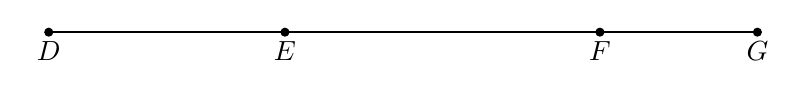
\begin{tikzpicture}
        \draw [-, thick] (0,0)--(9,0);
        \draw [fill] (0,0) circle [radius=0.05] node[below]{$D$};
        \draw [fill] (3,0) circle [radius=0.05] node[below]{$E$};
        \draw [fill] (7,0) circle [radius=0.05] node[below]{$F$};
        \draw [fill] (9,0) circle [radius=0.05] node[below]{$G$};
      \end{tikzpicture}
    \end{flushleft} \vspace{1cm}

\item Given $\overline{FG}$ as shown. What is the distance on the number line between the points?\\[1cm]
  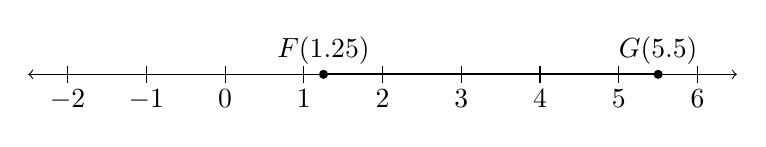
\begin{tikzpicture}
    \draw [<->] (-2.5,0)--(6.5,0);
    \foreach \x in {-2,...,6} %2 leading for diff!=1
      \draw[shift={(\x,0)},color=black] (0pt,-3pt) -- (0pt,3pt) node[below=5pt]  {$\x$};
      \draw [thick] (1.25,0)--(5.5,0);
      \draw [fill] (1.25,0) circle [radius=0.05] node[above] {$F(1.25)$};
      \draw [fill] (5.5,0) circle [radius=0.05] node[above] {$G(5.5)$};
  \end{tikzpicture} \vspace{1cm}

\item Given $\overline{RST}$, $RS=3 \frac{2}{3}$, and $RT=9 \frac{1}{3}$. Find ${ST}$ (expressed as a fraction, not a decimal).\\[1cm]
  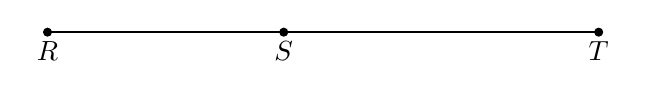
\begin{tikzpicture}
    \draw [-, thick] (0,0)--(7,0);
    \draw [fill] (0,0) circle [radius=0.05] node[below]{$R$};
    \draw [fill] (3,0) circle [radius=0.05] node[below]{$S$};
    \draw [fill] (7,0) circle [radius=0.05] node[below]{$T$};
  \end{tikzpicture} \vspace{2cm}

\item As shown below, two lines intersect making four angles: $\angle 1$, $\angle 2$, $\angle 3$, and $\angle 4$.
  \begin{center}
  \begin{tikzpicture}[scale=0.6]
    \draw [<->, thick] (0,-1.5)--(10,1.5);
    \draw [<->, thick] (2,3.5)--(7,-3.5);
    \node at (3,.4){1};
    \node at (6,-.6){3};
    \node at (5,1){2};
    \node at (4,-1){4};
    %\draw [fill] (0,0) circle [radius=0.05] node[below]{$P$};
    %\draw [fill] (6,0) circle [radius=0.05] node[below]{$R$};
    %\draw [fill] (3,0) circle [radius=0.05] node[below]{$Q$};
  \end{tikzpicture}
  \end{center}
  \begin{enumerate}
  \item Which angle is opposite $\angle 1$? \rule{4cm}{0.15mm} \bigskip
  \item Name an angle that is adjacent to $\angle 4$. \rule{4cm}{0.15mm} \bigskip
  \item True or false, $\angle 2$ and $\angle 4$ are vertical angles. \rule{3cm}{0.15mm}
\end{enumerate}

\newpage
\item Write the appropriate name for the type of angle depending on its measure in degrees. (acute, right, obtuse, or straight)
    \begin{enumerate}
      \item $m\angle = 90$ : \rule{4cm}{0.15mm} \bigskip
      \item $90 < m\angle < 180$ : \rule{4cm}{0.15mm} \bigskip
      \item $0< m\angle < 90$ : \rule{4cm}{0.15mm} \bigskip
      \item $m\angle = 180$ : \rule{4cm}{0.15mm} \bigskip
    \end{enumerate}

\item Given the diagram below. \vspace{0.25cm}
  \begin{enumerate}
    \item Name an angle that is vertical to $\angle DOE$: \rule{4cm}{0.15mm}
    \bigskip
    \item Name the ray that is opposite to $\overrightarrow{OB}$: \rule{4cm}{0.15mm}
    \bigskip
    \item Name an angle that is complementary to $\angle AOB$: \rule{4cm}{0.15mm} 
  \end{enumerate}
  \begin{center}
  \begin{tikzpicture}[scale=1, rotate=-20]
    \draw [<->, thick] (-55:3)--(0,0)--(125:4);
    \draw [<->, thick] (-5,0)--(5,0);
    \draw [->, thick] (0,0)--(0,4);
    \draw (0,0)++(0.3,0)--++(0,0.3)--+(-0.3,0);
    %\draw [fill] (-1,2.5) circle [radius=0.05] node[left ]{$B$};
    \draw [fill] (125:3) circle [radius=0.05] node[below left]{$B$};
    \draw [fill] (-4,0) circle [radius=0.05] node[below]{$A$}; 
    \draw [fill] (0,0) circle [radius=0.05] node[below left]{$O$};
    \draw [fill] (0,3) circle [radius=0.05] node[left]{$C$};
    \draw [fill] (4,0) circle [radius=0.05] node[below]{$D$};
    \draw [fill] (-55:2) circle [radius=0.05] node[left]{$E$};
  \end{tikzpicture}
  \end{center}

\item Given isosceles $\triangle XYZ$ with $\overline{XY} \cong \overline{XZ}$. On the diagram mark the congruent line segments with tick marks.
  \begin{center}
  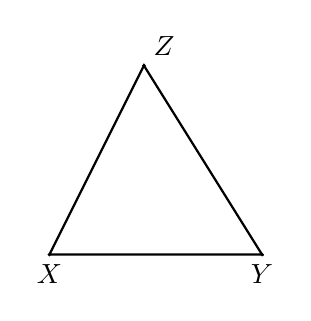
\begin{tikzpicture}[scale=0.3]
    \draw [thick](0,0)--(9,0)--(4,8)--(0,0);
    \draw [fill] (0,0) circle [radius=0.05] node[below]{$X$};
    \draw [fill] (9,0) circle [radius=0.05] node[below]{$Y$};
    \draw [fill] (4,8) circle [radius=0.05] node[above right]{$Z$};
  \end{tikzpicture}
  \end{center}

\end{enumerate}
\end{document}